\chapter{功能介绍}

\section{数学公式}

比如\autoref{eq:1}是单行公式
\begin{equation}
    \label{eq:1}
    \int_{-\infty}^{+\infty} e^{-x^2} dx = \sqrt{\pi}
\end{equation}
而\autoref{eq:2}是多行公式。注意如果这些公式应当在同一段内,在\texttt{equation}环境前后不要有空行,这样后续文本才不会被认为是下一段,从而有首行缩进。如果你觉得这样太乱了,可以在文本与公式行间加个\texttt{\%}隔开。
%
\begin{equation}\label{eq:2}
    \begin{aligned}
        & \tau_{12}=\tau_1-\tau_2=\frac{r_1-r_2}{c}; \\
        & \tau_{23}=\tau_2-\tau_3=\frac{r_2-r_3}{c}; \\
        & \tau_{13}=\tau_{12} + \tau_{23}            \\
    \end{aligned}
\end{equation}

\section{图片}

比如\autoref{fig:pngtest}. 注意模板中已经默认设置figure及table环境的位置参数为\texttt{htb} (优先放在当前位置, 其次放在页面顶部, 再次放在页面底部), 不能再单独设置. 另外在figure及table环境开头插入\mintinline{latex}{\centering},即已经默认图/表居中.
\begin{figure}
    \includegraphics[width=0.5\textwidth]{pngtest}
    \bicaption{ucasthesis 图片测试}{ucasthesis figure test}\label{fig:pngtest}
\end{figure}

如果想要绘制矢量图,推荐用\url{https://www.draw.io/}绘制图形,支持导出\textbf{仅绘图范围}的图形为pdf。由于\LaTeX 对svg支持不好,因此pdf格式是在\LaTeX 中插入矢量图片的最佳选择。导出时需将范围选为\textbf{裁剪},边框宽度设为0。不勾选包含绘图副本能让导出的pdf更小。

\section{表格}

有\texttt{tabular}和\texttt{tabularx}两个环境可以用于创建表格,主要区别在于\texttt{tabularx}提供了一个特殊的列类型 X,可以根据表格总宽度自动调整列宽。然而,在大多情况下表格宽度明显小于页面宽度,其实\texttt{tabular}更为合适。\autoref{tab:sample}是一个\texttt{tabular}环境创建的表格,\verb|>{\centering\arraybackslash}p{2\ccwd}|可以创建限定列宽又使单元格内容居中的列,需要注意此列中只能手动换行。其中,\verb|\ccwd|是一个汉字的宽度,也即约两英文字母宽度。
\begin{table}
    \bicaption{这是一个样表}{This is a sample table}\label{tab:sample}
    \begin{tabular}{
        l
        p{8\ccwd}
        c
        >{\centering\arraybackslash}p{2\ccwd}
        >{\centering\arraybackslash}p{3\ccwd}
    }
        \toprule
        指标 & 方法1 & 方法2 & 限制\newline 列宽 &同时\newline 能居中\\
        \midrule
        呵呵呵 &\texttt{tabular}中指定列宽的p类列可以自动换行 &124 &1234 & 1234567\\
        哈哈哈 &也可以用\newline\texttt{\textbackslash{newline}}\newline{}手动换行 & 1234567890 & 123 & 123 \\
        \bottomrule
    \end{tabular}
\end{table}

\begin{table}
    \bicaption{这样本身就比较宽的表我觉得才适合用\texttt{tabularx}创建,最右列类型为l能让最后一列对齐表格右边界}{Bla bla bla}\label{tab:another-sample}
    \begin{tabularx}{\textwidth}{cXXl}
        \toprule
        指标        &xxx    &xxx    &xxxxxx	\\
        \midrule
        代表产品    &xxxxxxxxxx   &xxxxxxxxxxxxxx  &xxxxxxxxxxxxxxxxxx \\
        xxxx    &xxxxxxxxx & xxxxxxx   &xxx \\
        xxxxxxxxx &xxxxx    &xxxx      &xxxxx \\
        xxxxxxxxx &xxxxxxxxxxxxxxx    &xxxxxxxxxxxxxx     &xxxxxxx \\
        \bottomrule
    \end{tabularx}
\end{table}

\section{术语}

有符号: \gls{pi}, 有缩写: \gls{spi}。缩写首次出现会给出中文及英文全程,后续出现只给出缩写本身,比如\gls{spi}。在\path{bibs/symbols.bib}添加你的符号,在\path{bibs/abbreviations.bib}添加你的缩写。

\section{引用}

将你要引用的文献的biblatex条目(bibtex格式也可以,前者更佳)添加到\path{bibs/references.bib}中,从而能在文中引用。不建议手打biblatex,费时费力且容易搞错格式,可以从谷歌学术中复制,或利用Zotero Connector等进行抓取。

本模板使用biber进行文献编译,基本符合2015国标的参考文献格式。默认情况下,按照国科大的指导标准,使用数字顺序的引用方式没有严格限制,这也是最方便的引用途径。 如果您一定要使用作者年份制引用,请参照参考文献模板的说明进行使用。

看看这个例子,关于书的\cite{tex, companion, ColdSources},还有这些\cite{Krasnogor2004e, clzs,zjsw},关于杂志的\cite{ELIDRISSI94, MELLINGER96, SHELL02},硕士论文\cite{zhubajie, metamori2004},博士论文\cite{shaheshang, FistSystem01},标准文件\cite{IEEE-1363},会议论文\cite{DPMG,kocher99},技术报告\cite{NPB2}。中文参考文献\cite{cnarticle}应增加 \texttt{lang=``zh''} 字段,以便进行相应处理。更多参考文献模板使用方法请参照参考文献模板作者说明\url{https://github.com/hushidong/biblatex-gb7714-2015}。

\section{常用符号}
模板引入了\texttt{gensymb}宏包,提供一些科学和数学中常用的通用符号,如各种单位符号:
\begin{itemize}
    \item \verb|\degree|: 角度\degree
    \item \verb|\celsius|: 摄氏度\celsius
    \item \verb|\ohm|: 欧姆\ohm
\end{itemize}

\section{tikz绘图}

可以在\url{https://www.mathcha.io/editor}中创建文档后选择Insert Diagram 中的Drawing Area,绘制图形。焦点在该绘图区域中时顶部工具栏中有导出为Tikz代码的选项,复制后粘贴到\LaTeX 工程中一个单独的tex文件,并将这个文件作为图片插入文中。注意\texttt{tikzpicture}环境的\texttt{xscale}/\texttt{yscale}参数可以缩放整个图形,\texttt{every node}命令可以设置所有节点的字体大小。\autoref{fig:near_field}是一个例子。

\begin{figure}
    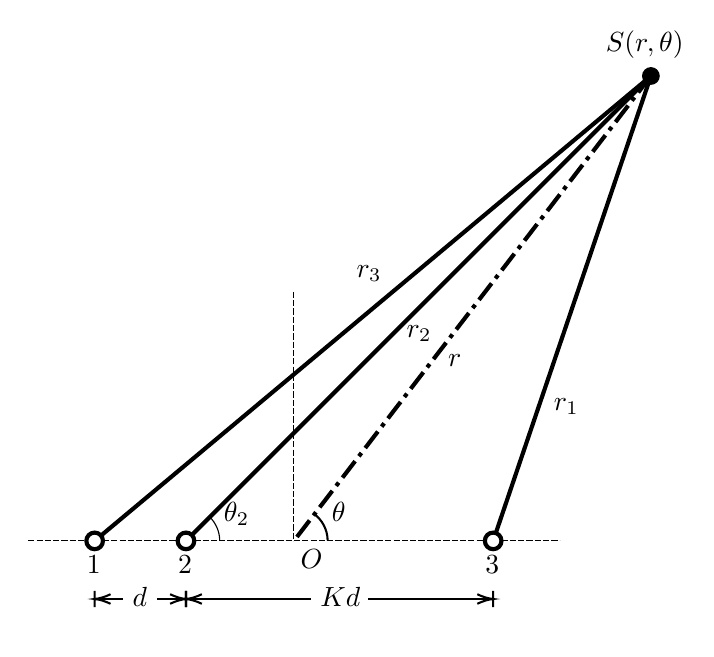
\begin{tikzpicture}[every picture/.style={line width=0.75pt}, x=0.75pt,y=0.75pt,yscale=-1,xscale=1]
    %uncomment if require: \path (0,318); %set diagram left start at 0, and has height of 318

    %Straight Lines [id:da042324791837329956]
    \draw [line width=1.5]    (244,268) -- (468,44) ;
    %Straight Lines [id:da7482650625206233]
    \draw [line width=1.5]    (468,44) -- (392,268) ;
    %Straight Lines [id:da8759803470570984]
    \draw  [dash pattern={on 2.25pt off 0.75pt}]  (168,268) -- (424,268) ;
    %Straight Lines [id:da3612564917664043]
    \draw  [dash pattern={on 2.25pt off 0.75pt}]  (296,148) -- (296,268) ;

    %Shape: Circle [id:dp701214228276472]
    \draw  [fill={rgb, 255:red, 0; green, 0; blue, 0 }  ,fill opacity=1 ] (464,44) .. controls (464,41.79) and (465.79,40) .. (468,40) .. controls (470.21,40) and (472,41.79) .. (472,44) .. controls (472,46.21) and (470.21,48) .. (468,48) .. controls (465.79,48) and (464,46.21) .. (464,44) -- cycle ;
    %Straight Lines [id:da46776944434905854]
    \draw [line width=1.5]    (468,44) -- (200,268) ;
    %Shape: Circle [id:dp41637404945939793]
    \draw  [fill={rgb, 255:red, 255; green, 255; blue, 255 }  ,fill opacity=1 ][line width=1.5]  (388,268) .. controls (388,265.79) and (389.79,264) .. (392,264) .. controls (394.21,264) and (396,265.79) .. (396,268) .. controls (396,270.21) and (394.21,272) .. (392,272) .. controls (389.79,272) and (388,270.21) .. (388,268) -- cycle ;
    %Shape: Circle [id:dp3472405999942534]
    \draw  [fill={rgb, 255:red, 255; green, 255; blue, 255 }  ,fill opacity=1 ][line width=1.5]  (196,268) .. controls (196,265.79) and (197.79,264) .. (200,264) .. controls (202.21,264) and (204,265.79) .. (204,268) .. controls (204,270.21) and (202.21,272) .. (200,272) .. controls (197.79,272) and (196,270.21) .. (196,268) -- cycle ;
    %Straight Lines [id:da8463556712184459]
    \draw [line width=1.5]  [dash pattern={on 7.5pt off 2.25pt on 1.5pt off 2.25pt}]  (468,44) -- (296,268) ;
    %Shape: Arc [id:dp41353820710334777]
    \draw  [draw opacity=0][line width=0.75]  (305.66,254.93) .. controls (309.58,257.84) and (312.15,262.46) .. (312.25,267.68) -- (296,268) -- cycle ; \draw  [line width=0.75]  (305.66,254.93) .. controls (309.58,257.84) and (312.15,262.46) .. (312.25,267.68) ;
    %Shape: Arc [id:dp19292277101405086]
    \draw  [draw opacity=0] (255.44,256.46) .. controls (258.34,259.33) and (260.16,263.29) .. (260.25,267.68) -- (244,268) -- cycle ; \draw   (255.44,256.46) .. controls (258.34,259.33) and (260.16,263.29) .. (260.25,267.68) ;
    %Straight Lines [id:da8674403841051044]
    \draw    (200,296) -- (244,296) ;
    \draw [shift={(244,296)}, rotate = 180] [color={rgb, 255:red, 0; green, 0; blue, 0 }  ][line width=0.75]    (0,3.91) -- (0,-3.91)(7.65,-2.3) .. controls (4.86,-0.97) and (2.31,-0.21) .. (0,0) .. controls (2.31,0.21) and (4.86,0.98) .. (7.65,2.3)   ;
    \draw [shift={(200,296)}, rotate = 0] [color={rgb, 255:red, 0; green, 0; blue, 0 }  ][line width=0.75]    (0,3.91) -- (0,-3.91)(7.65,-2.3) .. controls (4.86,-0.97) and (2.31,-0.21) .. (0,0) .. controls (2.31,0.21) and (4.86,0.98) .. (7.65,2.3)   ;
    %Shape: Circle [id:dp45604077591200665]
    \draw  [fill={rgb, 255:red, 255; green, 255; blue, 255 }  ,fill opacity=1 ][line width=1.5]  (240,268) .. controls (240,265.79) and (241.79,264) .. (244,264) .. controls (246.21,264) and (248,265.79) .. (248,268) .. controls (248,270.21) and (246.21,272) .. (244,272) .. controls (241.79,272) and (240,270.21) .. (240,268) -- cycle ;
    %Straight Lines [id:da3454693803086273]
    \draw    (244,296) -- (392,296) ;
    \draw [shift={(392,296)}, rotate = 180] [color={rgb, 255:red, 0; green, 0; blue, 0 }  ][line width=0.75]    (0,3.91) -- (0,-3.91)(7.65,-2.3) .. controls (4.86,-0.97) and (2.31,-0.21) .. (0,0) .. controls (2.31,0.21) and (4.86,0.98) .. (7.65,2.3)   ;
    \draw [shift={(244,296)}, rotate = 0] [color={rgb, 255:red, 0; green, 0; blue, 0 }  ][line width=0.75]    (0,3.91) -- (0,-3.91)(7.65,-2.3) .. controls (4.86,-0.97) and (2.31,-0.21) .. (0,0) .. controls (2.31,0.21) and (4.86,0.98) .. (7.65,2.3)   ;

    % Text Node
    \draw (387,274) node [anchor=north west][inner sep=0.75pt]   [align=left] {3};
    % Text Node
    \draw (195,274) node [anchor=north west][inner sep=0.75pt]   [align=left] {1};
    % Text Node
    \draw (420,198) node [anchor=north west][inner sep=0.75pt]   [align=left] {$\displaystyle r_{1}$};
    % Text Node
    \draw (349,163) node [anchor=north west][inner sep=0.75pt]   [align=left] {$\displaystyle r_{2}$};
    % Text Node
    \draw (325,134) node [anchor=north west][inner sep=0.75pt]   [align=left] {$\displaystyle r_{3}$};
    % Text Node
    \draw (369,177) node [anchor=north west][inner sep=0.75pt]   [align=left] {$\displaystyle r$};
    % Text Node
    \draw (313,248) node [anchor=north west][inner sep=0.75pt]   [align=left] {$\displaystyle \theta $};
    % Text Node
    \draw (261,248) node [anchor=north west][inner sep=0.75pt]   [align=left] {$\displaystyle \theta _{2}$};
    % Text Node
    \draw (445,21) node [anchor=north west][inner sep=0.75pt]   [align=left] {$\displaystyle S( r,\theta )$};
    % Text Node
    \draw  [color={rgb, 255:red, 255; green, 255; blue, 255 }  ,draw opacity=1 ][fill={rgb, 255:red, 255; green, 255; blue, 255 }  ,fill opacity=1 ]  (214,285) -- (230,285) -- (230,310) -- (214,310) -- cycle  ;
    \draw (217,289) node [anchor=north west][inner sep=0.75pt]   [align=left] {$\displaystyle d$};
    % Text Node
    \draw  [color={rgb, 255:red, 255; green, 255; blue, 255 }  ,draw opacity=1 ][fill={rgb, 255:red, 255; green, 255; blue, 255 }  ,fill opacity=1 ]  (304.5,285) -- (331.5,285) -- (331.5,310) -- (304.5,310) -- cycle  ;
    \draw (307.5,289) node [anchor=north west][inner sep=0.75pt]   [align=left] {$\displaystyle Kd$};
    % Text Node
    \draw (298,271) node [anchor=north west][inner sep=0.75pt]   [align=left] {$\displaystyle O$};
    % Text Node
    \draw (239,274) node [anchor=north west][inner sep=0.75pt]   [align=left] {2};


\end{tikzpicture}
    \bicaption{近场几何模型}{near-field source geometry}\label{fig:near_field}
\end{figure}

\section{代码}

代码可以是行内的, 如\mintinline{python3}{print('是字符串' if isinstance(aString, str) else '不是字符串')}, 可以是单行的:
\mint{tex}{\inputminted[firstline=16, lastline=37]{c}{assets/example.c}}
也可以是如下从指定文件指定范围插入的代码块\autoref{code:sample}。
\begin{listing}[H]
    \inputminted[firstline=26, lastline=37]{c}{assets/example.c}
    \bicaption{这是一段示例代码}{A sample code}\label{code:sample}
\end{listing}

\section{算法}

\autoref{alg:alg1}是基于\texttt{algpseudocode}包实现的伪代码示例。注意编写自己的伪代码时不要错误地使用了algorithmic包提供的伪代码命令。

\path{styles/ucasDissertation.cls}中\mintinline{latex}{\RequirePackage{algpseudocode}}行后一段覆写了伪代码关键字的显示文本以实现汉化。

\begin{algorithm}
    \caption{计算 $y = x^n$}\label{alg:alg1}
    \begin{algorithmic}[1]  % 参数[1]表示显示行号
        \Require $n \geq 0 \vee x \neq 0$
        \Ensure $y = x^n$

        % 初始化
        \State $y \gets 1$

        % 逻辑
        \If{$n < 0$}
            \State $X \gets 1 / x$
            \State $N \gets -n$
        \Else
            \State $X \gets x$
            \State $N \gets n$
        \EndIf

        \While{$N \neq 0$}
            \If{$N$ 是偶数}
                \State $X \gets X \times X$
                \State $N \gets N / 2$
            \ElsIf{$N$ 是奇数}
                \State $y \gets y \times X$
                \State $N \gets N - 1$
            \EndIf
        \EndWhile
    \end{algorithmic}
\end{algorithm}